% UAI 2026 Presentation: Diagnosing Conformal Prediction Failures Under Distribution Shift
% Author: Chorok Lee, KAIST
% Date: August 17-21, 2026, Amsterdam

\documentclass[aspectratio=169,11pt]{beamer}

% Theme and colors
\usetheme{Madrid}
\usecolortheme{default}
\definecolor{kaistblue}{RGB}{0,51,102}
\definecolor{alertred}{RGB}{178,34,34}
\definecolor{successgreen}{RGB}{34,139,34}
\setbeamercolor{structure}{fg=kaistblue}
\setbeamercolor{alerted text}{fg=alertred}

% Packages
\usepackage{amsmath,amssymb,amsthm}
\usepackage{graphicx}
\usepackage{booktabs}
\usepackage{tikz}
\usetikzlibrary{shapes,arrows,positioning,calc}
\usepackage{algorithm}
\usepackage{algorithmic}
\usepackage{xcolor}

% Custom commands
\newcommand{\rmark}{\textcolor{alertred}{\ding{55}}}
\newcommand{\gmark}{\textcolor{successgreen}{\ding{51}}}
\newcommand{\conc}{\mathcal{H}}
\newcommand{\cov}{\mathcal{C}}

% Remove navigation symbols
\setbeamertemplate{navigation symbols}{}

% Slide numbers
\setbeamertemplate{footline}[frame number]

% Title information
\title[SHAP Concentration \& CP Failures]{Diagnosing Conformal Prediction Failures\\Under Distribution Shift}
\subtitle{A COVID-19 Case Study}
\author[Chorok Lee]{Chorok Lee}
\institute[KAIST]{Korea Advanced Institute of Science and Technology (KAIST)}
\date{UAI 2026 \\ Amsterdam, August 17--21}

\begin{document}

%==============================================================================
% TITLE SLIDE
%==============================================================================
\begin{frame}
\titlepage
\end{frame}

%==============================================================================
% MOTIVATION/PROBLEM (Slides 2-4)
%==============================================================================

\begin{frame}{The Promise of Conformal Prediction}

\begin{columns}
\begin{column}{0.55\textwidth}
\textbf{Conformal Prediction} provides:
\vspace{1em}
\begin{itemize}
    \item[$\checkmark$] \alert{Distribution-free} coverage guarantees
    \item[$\checkmark$] Works with \textbf{any} base model
    \item[$\checkmark$] Exact finite-sample validity
\end{itemize}

\vspace{1.5em}
\textbf{Target:} 90\% coverage ($\alpha = 0.1$)

\vspace{0.5em}
$\Rightarrow$ True label in prediction set at least 90\% of the time
\end{column}

\begin{column}{0.45\textwidth}
% Placeholder for figure
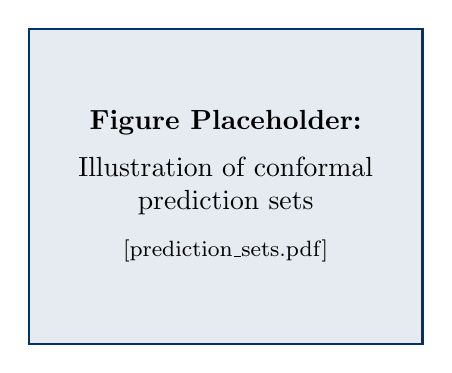
\begin{tikzpicture}
\draw[thick,kaistblue,fill=kaistblue!10] (0,0) rectangle (5,4);
\node[align=center] at (2.5,2) {
    \textbf{Figure Placeholder:}\\[0.5em]
    Illustration of conformal\\
    prediction sets\\[0.5em]
    \footnotesize{[prediction\_sets.pdf]}
};
\end{tikzpicture}
\end{column}
\end{columns}

\vspace{1em}
\centering
\textit{But there's a catch...}
\end{frame}

%------------------------------------------------------------------------------

\begin{frame}{The Hidden Assumption}

\begin{center}
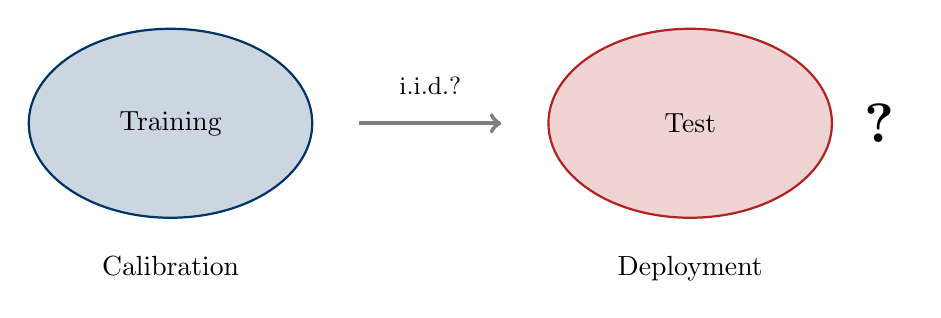
\begin{tikzpicture}[scale=1.2]
% Training distribution
\draw[thick,kaistblue,fill=kaistblue!20] (0,0) ellipse (1.5 and 1);
\node at (0,0) {Training};
\node[below] at (0,-1.3) {Calibration};

% Arrow
\draw[->,ultra thick,gray] (2,0) -- (3.5,0);
\node[above] at (2.75,0.2) {\small i.i.d.?};

% Test distribution
\draw[thick,alertred,fill=alertred!20] (5.5,0) ellipse (1.5 and 1);
\node at (5.5,0) {Test};
\node[below] at (5.5,-1.3) {Deployment};

% Question mark
\node[scale=2] at (7.5,0) {\textbf{?}};
\end{tikzpicture}
\end{center}

\vspace{1em}

\begin{alertblock}{The Exchangeability Assumption}
Conformal prediction \textbf{requires} calibration and test data to be exchangeable (approximately i.i.d.)
\end{alertblock}

\vspace{0.5em}

\textbf{Problem:} In real-world deployments, \alert{distribution shift is inevitable}

\begin{itemize}
    \item Temporal shift (COVID-19 changing behavior patterns)
    \item Geographic shift (new regions)
    \item Demographic shift (new user populations)
\end{itemize}

\end{frame}

%------------------------------------------------------------------------------

\begin{frame}{The Research Gap}

\begin{columns}
\begin{column}{0.5\textwidth}
\textbf{Standard Shift Detectors:}
\vspace{0.5em}
\begin{itemize}
    \item MMD (Maximum Mean Discrepancy)
    \item C2ST (Classifier Two-Sample Test)
    \item PSI (Population Stability Index)
\end{itemize}

\vspace{1em}
\textcolor{alertred}{\textbf{Their limitation:}}\\
Detect shift \textbf{uniformly} across all tasks

\vspace{0.5em}
$\Rightarrow$ Cannot distinguish:
\begin{itemize}
    \item \textcolor{successgreen}{Robust outcomes} (coverage OK)
    \item \textcolor{alertred}{Catastrophic failures} (coverage broken)
\end{itemize}
\end{column}

\begin{column}{0.5\textwidth}
% Placeholder for comparison figure
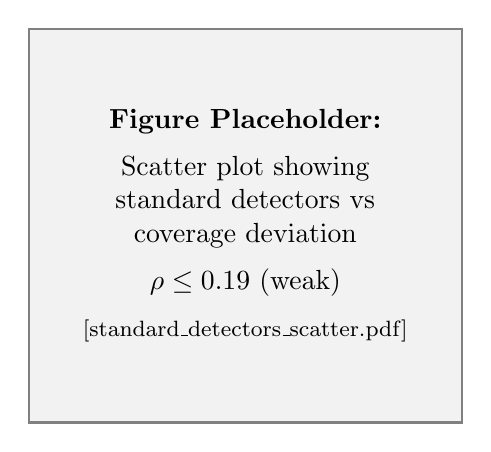
\begin{tikzpicture}
\draw[thick,gray,fill=gray!10] (0,0) rectangle (5.5,5);
\node[align=center] at (2.75,2.5) {
    \textbf{Figure Placeholder:}\\[0.5em]
    Scatter plot showing\\
    standard detectors vs\\
    coverage deviation\\[0.5em]
    $\rho \leq 0.19$ (weak)\\[0.5em]
    \footnotesize{[standard\_detectors\_scatter.pdf]}
};
\end{tikzpicture}
\end{column}
\end{columns}

\vspace{1em}
\centering
\fbox{\textbf{Research Question:} Can we \textit{predict} when conformal prediction will fail?}
\end{frame}

%==============================================================================
% BACKGROUND ON CONFORMAL PREDICTION (Slides 5-6)
%==============================================================================

\begin{frame}{Conformal Prediction: A Brief Primer}

\textbf{Setup:} Classification with $K$ classes, base model outputs $\hat{\pi}(y|x)$

\vspace{1em}

\begin{columns}
\begin{column}{0.48\textwidth}
\textbf{1. Define nonconformity score}
\vspace{0.3em}

For \alert{Adaptive Prediction Sets (APS)}:
$$s(x,y) = \sum_{k: \hat{\pi}_k \geq \hat{\pi}_y} \hat{\pi}_k$$

\vspace{0.3em}
\footnotesize{(Sum of probabilities of classes ranked above true class)}
\end{column}

\begin{column}{0.48\textwidth}
\textbf{2. Calibrate threshold}
\vspace{0.3em}

From calibration set $\{(x_i, y_i)\}_{i=1}^n$:
$$\hat{q} = \text{Quantile}_{1-\alpha}\left(\{s(x_i, y_i)\}_{i=1}^n\right)$$
\end{column}
\end{columns}

\vspace{1em}

\begin{columns}
\begin{column}{0.48\textwidth}
\textbf{3. Form prediction sets}
\vspace{0.3em}

$$\mathcal{C}(x) = \{y : s(x,y) \leq \hat{q}\}$$
\end{column}

\begin{column}{0.48\textwidth}
\textbf{4. Coverage guarantee}
\vspace{0.3em}

$$\mathbb{P}(Y \in \mathcal{C}(X)) \geq 1 - \alpha$$
\textcolor{gray}{\footnotesize (Under exchangeability)}
\end{column}
\end{columns}

\vspace{1em}
\centering
\textit{We use $\alpha = 0.1$ throughout (target: 90\% coverage)}
\end{frame}

%------------------------------------------------------------------------------

\begin{frame}{What Happens Under Distribution Shift?}

\begin{center}
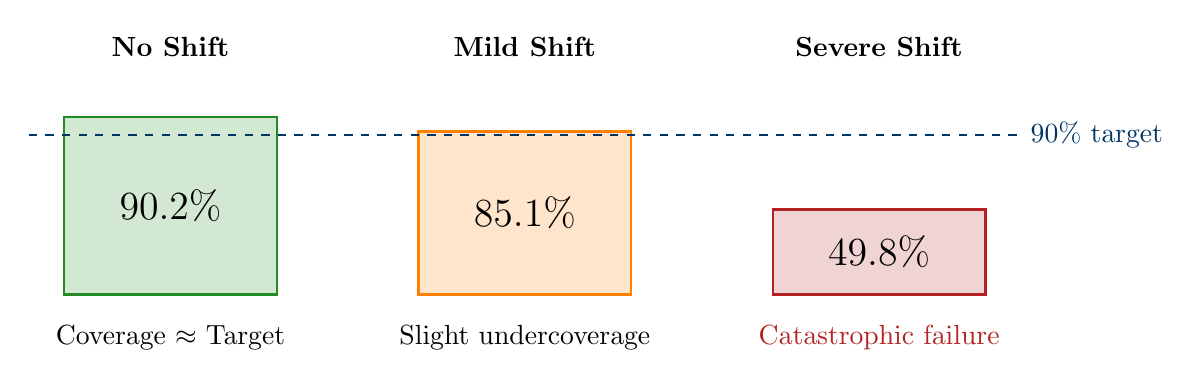
\begin{tikzpicture}[scale=0.9]
% Left side - good coverage
\node[align=center] at (0,3.5) {\textbf{No Shift}};
\draw[thick,successgreen,fill=successgreen!20] (-1.5,0) rectangle (1.5,2.5);
\node at (0,1.25) {\Large 90.2\%};
\node[below] at (0,-0.3) {Coverage $\approx$ Target};

% Middle - mild
\node[align=center] at (5,3.5) {\textbf{Mild Shift}};
\draw[thick,orange,fill=orange!20] (3.5,0) rectangle (6.5,2.3);
\node at (5,1.15) {\Large 85.1\%};
\node[below] at (5,-0.3) {Slight undercoverage};

% Right - catastrophic
\node[align=center] at (10,3.5) {\textbf{Severe Shift}};
\draw[thick,alertred,fill=alertred!20] (8.5,0) rectangle (11.5,1.2);
\node at (10,0.6) {\Large 49.8\%};
\node[below] at (10,-0.3) {\textcolor{alertred}{Catastrophic failure}};

% Target line
\draw[dashed,thick,kaistblue] (-2,2.25) -- (12,2.25);
\node[right,kaistblue] at (12,2.25) {90\% target};
\end{tikzpicture}
\end{center}

\vspace{1em}

\begin{alertblock}{Key Observation}
Distribution shift severity alone does \textbf{not} predict coverage failure.\\
\textbf{What matters is \textit{how} features shift relative to model reliance.}
\end{alertblock}

\end{frame}

%------------------------------------------------------------------------------

\begin{frame}{Conformal Prediction Pipeline}

\begin{center}
% CP Methodology Pipeline Figure (FigureLabs generated)

\includegraphics[width=0.95\textwidth]{figures/fig2_cp_methodology.jpg}
\end{center}

\vspace{0.3em}
\centering
\textit{Under distribution shift: calibrated threshold becomes invalid $\Rightarrow$ coverage breaks}

\end{frame}

%==============================================================================
% OUR APPROACH: SHAP CONCENTRATION (Slides 7-9)
%==============================================================================

\begin{frame}{Our Key Insight}

\begin{center}
\Large
\textit{``The vulnerability of conformal prediction is determined by}\\
\textit{how \textbf{concentrated} the model's reliance is on shifting features.''}
\end{center}

\vspace{1.5em}

\begin{columns}
\begin{column}{0.5\textwidth}
\centering
\textbf{Low Concentration}\\[0.5em]
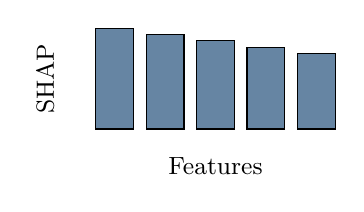
\begin{tikzpicture}[scale=0.8]
\foreach \i/\h in {1/0.8, 2/0.75, 3/0.7, 4/0.65, 5/0.6} {
    \draw[fill=kaistblue!60] (\i*0.8-0.3,0) rectangle (\i*0.8+0.3,\h*2);
}
\node[below] at (2.4,-0.3) {\small Features};
\node[rotate=90] at (-0.3,0.8) {\small SHAP};
\end{tikzpicture}
\\[0.5em]
$\Rightarrow$ \textcolor{successgreen}{\textbf{Robust}}
\end{column}

\begin{column}{0.5\textwidth}
\centering
\textbf{High Concentration}\\[0.5em]
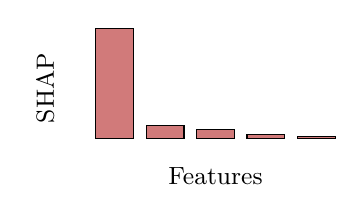
\begin{tikzpicture}[scale=0.8]
\foreach \i/\h in {1/2.5, 2/0.3, 3/0.2, 4/0.1, 5/0.05} {
    \draw[fill=alertred!60] (\i*0.8-0.3,0) rectangle (\i*0.8+0.3,\h*0.7);
}
\node[below] at (2.4,-0.3) {\small Features};
\node[rotate=90] at (-0.3,0.8) {\small SHAP};
\end{tikzpicture}
\\[0.5em]
$\Rightarrow$ \textcolor{alertred}{\textbf{Vulnerable}}
\end{column}
\end{columns}

\vspace{1em}
\centering
We measure concentration using \alert{Shannon entropy} of SHAP importance distribution
\end{frame}

%------------------------------------------------------------------------------

\begin{frame}{SHAP Concentration: The Metric}

\textbf{Step 1:} Compute mean absolute SHAP values on validation data
$$\phi_j = \frac{1}{n}\sum_{i=1}^{n}|\text{SHAP}_j(x_i)| \quad \text{for each feature } j$$

\vspace{0.8em}

\textbf{Step 2:} Compute \alert{SHAP Concentration} --- fraction in top feature
\begin{equation*}
\boxed{C = \frac{\phi_1}{\sum_{j=1}^{p} \phi_j}}
\end{equation*}
where $\phi_1$ is the importance of the \textbf{top-ranked} feature.

\vspace{1em}

\begin{columns}
\begin{column}{0.5\textwidth}
\centering
\textbf{Low $C$ ($<$ 40\%)}\\[0.3em]
Importance spread across features\\
\textcolor{successgreen}{\textbf{$\Rightarrow$ Robust to shift}}
\end{column}
\begin{column}{0.5\textwidth}
\centering
\textbf{High $C$ ($\geq$ 40\%)}\\[0.3em]
Single feature dominates\\
\textcolor{alertred}{\textbf{$\Rightarrow$ Vulnerable to shift}}
\end{column}
\end{columns}

\vspace{0.5em}
\centering
\textit{Simple, interpretable, computed \textbf{before} deployment}
\end{frame}

%------------------------------------------------------------------------------

\begin{frame}{Why Does Concentration Matter?}

\begin{columns}
\begin{column}{0.55\textwidth}
\textbf{Intuition:}
\vspace{0.5em}

When model relies on \textbf{few features}:
\begin{itemize}
    \item Shift in those features $\Rightarrow$ \alert{large score perturbation}
    \item Calibrated threshold becomes invalid
    \item Coverage collapses
\end{itemize}

\vspace{1em}

When model relies on \textbf{many features}:
\begin{itemize}
    \item Shift averages out across features
    \item Score distribution more stable
    \item Coverage maintained
\end{itemize}

\vspace{1em}
$\Rightarrow$ \alert{Concentration = fragility amplifier}
\end{column}

\begin{column}{0.45\textwidth}
% Placeholder for intuition diagram
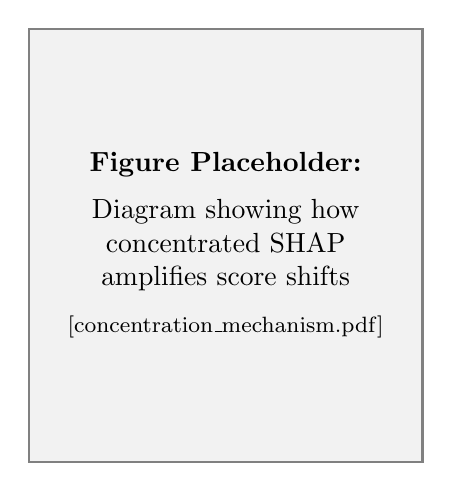
\begin{tikzpicture}
\draw[thick,gray,fill=gray!10] (0,0) rectangle (5,5.5);
\node[align=center] at (2.5,2.75) {
    \textbf{Figure Placeholder:}\\[0.5em]
    Diagram showing how\\
    concentrated SHAP\\
    amplifies score shifts\\[0.5em]
    \footnotesize{[concentration\_mechanism.pdf]}
};
\end{tikzpicture}
\end{column}
\end{columns}
\end{frame}

%==============================================================================
% METHODOLOGY (Slides 10-11)
%==============================================================================

\begin{frame}{Experimental Setup: SALT Benchmark}

\begin{columns}
\begin{column}{0.5\textwidth}
\textbf{SALT Benchmark:}
\begin{itemize}
    \item 8 e-commerce classification tasks
    \item \alert{COVID-19 temporal split}
    \begin{itemize}
        \item Calibration: Pre-COVID
        \item Test: During COVID
    \end{itemize}
    \item Natural distribution shift
\end{itemize}

\vspace{1em}

\textbf{Tasks:}
\begin{enumerate}
    \item Seller return rate
    \item Product conversion
    \item Delivery delay
    \item Customer churn
    \item ... (4 more)
\end{enumerate}
\end{column}

\begin{column}{0.5\textwidth}
% COVID Timeline Figure

\includegraphics[width=\textwidth]{figures/fig1_covid_timeline.jpg}
\end{column}
\end{columns}
\end{frame}

%------------------------------------------------------------------------------

\begin{frame}{Methodology Details}

\begin{columns}
\begin{column}{0.55\textwidth}
\textbf{Models:}
\begin{itemize}
    \item LightGBM (primary)
    \item CatBoost, XGBoost, Random Forest
\end{itemize}

\vspace{0.8em}

\textbf{Conformal Method:}
\begin{itemize}
    \item Adaptive Prediction Sets (APS)
    \item Target coverage: $1-\alpha = 90\%$
\end{itemize}

\vspace{0.8em}

\textbf{Statistical Robustness:}
\begin{itemize}
    \item 50 random seeds per experiment
    \item Spearman correlation with p-values
\end{itemize}

\vspace{0.8em}

\textbf{External Validation:}
\begin{itemize}
    \item 8 additional datasets (9 domains total)
    \item Covertype, MNIST-C, ImageNet-C, ...
\end{itemize}
\end{column}

\begin{column}{0.45\textwidth}
\begin{table}
\small
\centering
\begin{tabular}{lc}
\toprule
\textbf{Component} & \textbf{Setting} \\
\midrule
Calibration size & 1,000--5,000 \\
Test size & 5,000--50,000 \\
Features & 20--150 \\
Classes & 2--10 \\
$\alpha$ & 0.1 \\
Seeds & 50 \\
\bottomrule
\end{tabular}
\caption{Experimental parameters}
\end{table}
\end{column}
\end{columns}
\end{frame}

%==============================================================================
% MAIN RESULTS (Slides 12-16)
%==============================================================================

\begin{frame}{Main Result: Strong Correlation}

\begin{center}
% Main correlation scatter plot (FigureLabs generated)

\includegraphics[width=0.75\textwidth]{figures/fig3_correlation.jpg}
\end{center}

\vspace{0.3em}

\begin{alertblock}{Primary Finding}
SHAP concentration \textbf{strongly predicts} coverage failure severity\\
($\rho = 0.853$, $p < 0.001$, $n = 16$ tasks across 9 domains)
\end{alertblock}

\end{frame}

%------------------------------------------------------------------------------

\begin{frame}{Within SALT COVID Tasks}

\begin{columns}
\begin{column}{0.55\textwidth}
% Placeholder for SALT-specific plot
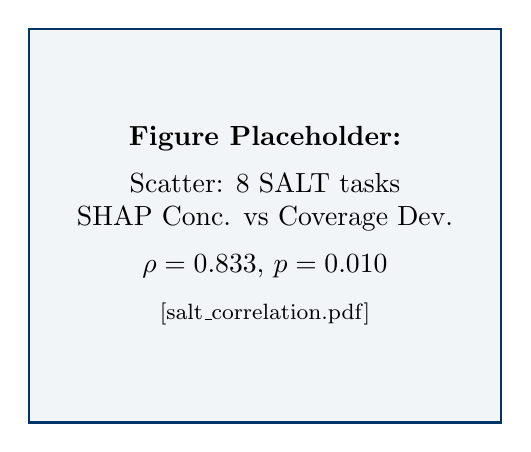
\begin{tikzpicture}
\draw[thick,kaistblue,fill=kaistblue!5] (0,0) rectangle (6,5);
\node[align=center] at (3,2.5) {
    \textbf{Figure Placeholder:}\\[0.5em]
    Scatter: 8 SALT tasks\\
    SHAP Conc. vs Coverage Dev.\\[0.5em]
    $\rho = 0.833$, $p = 0.010$\\[0.5em]
    \footnotesize{[salt\_correlation.pdf]}
};
\end{tikzpicture}
\end{column}

\begin{column}{0.45\textwidth}
\textbf{COVID Shift Results:}

\vspace{0.5em}
\begin{tabular}{@{}lcc@{}}
\toprule
Task & $\conc$ & Cov. \\
\midrule
Task A & 0.21 & 88.2\% \\
Task B & 0.28 & 85.7\% \\
Task C & 0.35 & 82.1\% \\
Task D & 0.42 & 78.3\% \\
Task E & 0.51 & 73.5\% \\
\textcolor{alertred}{Task F} & \textcolor{alertred}{0.67} & \textcolor{alertred}{65.2\%} \\
\bottomrule
\end{tabular}

\vspace{1em}
\footnotesize{Higher concentration $\Rightarrow$ worse coverage}
\end{column}
\end{columns}

\vspace{0.5em}
\centering
\textit{Correlation holds specifically within COVID-induced shifts}
\end{frame}

%------------------------------------------------------------------------------

\begin{frame}{Comparison: SHAP vs Standard Detectors}

\begin{center}
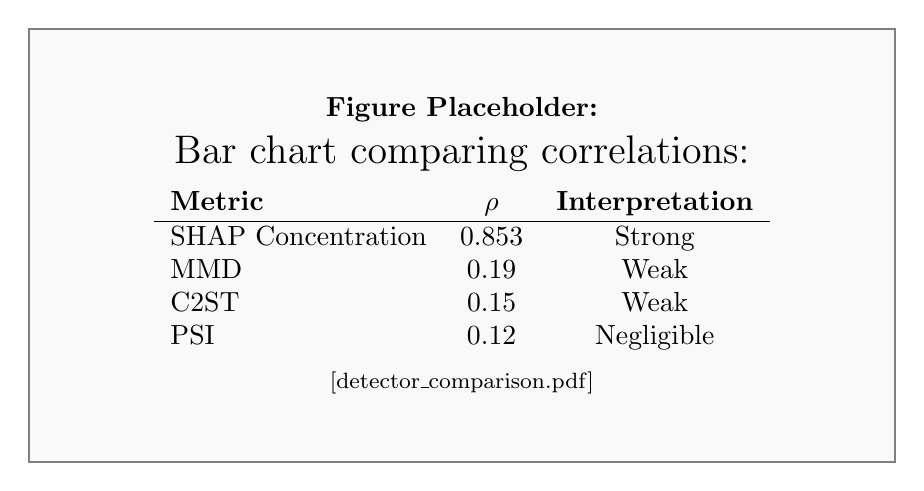
\begin{tikzpicture}
\draw[thick,gray,fill=gray!5] (0,0) rectangle (11,5.5);
\node[align=center] at (5.5,2.75) {
    \textbf{Figure Placeholder:}\\[0.5em]
    \Large Bar chart comparing correlations:\\[0.5em]
    \begin{tabular}{lcc}
    \textbf{Metric} & $\rho$ & \textbf{Interpretation} \\
    \hline
    \alert{SHAP Concentration} & \alert{0.853} & \alert{Strong} \\
    MMD & 0.19 & Weak \\
    C2ST & 0.15 & Weak \\
    PSI & 0.12 & Negligible \\
    \end{tabular}\\[0.5em]
    \footnotesize{[detector\_comparison.pdf]}
};
\end{tikzpicture}
\end{center}

\vspace{0.5em}

\begin{block}{Why Standard Detectors Fail}
They measure \textbf{marginal} distribution shift, not shift in \textbf{model-relevant} features.\\
All tasks show similar MMD/C2ST/PSI, but vastly different coverage outcomes.
\end{block}

\end{frame}

%------------------------------------------------------------------------------

\begin{frame}{External Validation: Covertype Geographic Shift}

\begin{columns}
\begin{column}{0.5\textwidth}
\textbf{Covertype Dataset:}
\begin{itemize}
    \item Forest cover type prediction
    \item 7 classes, 54 features
    \item \alert{Geographic split:} Areas 1--2 $\rightarrow$ Area 4
\end{itemize}

\vspace{1em}

\textbf{Results:}
\begin{itemize}
    \item SHAP Concentration: $C = 49.8\%$
    \item Target Coverage: 90\%
    \item \textcolor{alertred}{Actual Coverage: 8.2\%}
    \item \textcolor{alertred}{Coverage Drop: 81.8 pp}
\end{itemize}

\vspace{0.5em}
$\Rightarrow$ \alert{Catastrophic failure} correctly predicted!\\
\footnotesize{(10/10 seeds deterministic)}
\end{column}

\begin{column}{0.5\textwidth}
% Placeholder for covertype visualization
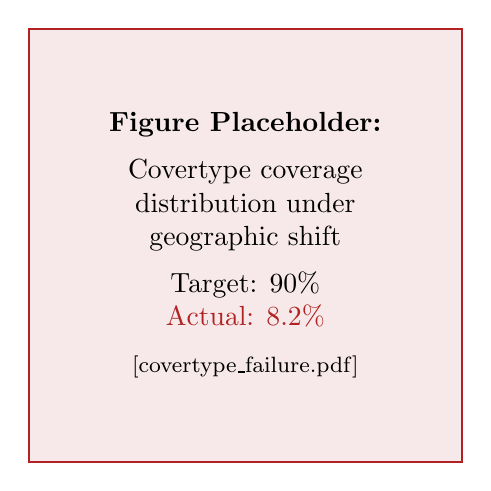
\begin{tikzpicture}
\draw[thick,alertred,fill=alertred!10] (0,0) rectangle (5.5,5.5);
\node[align=center] at (2.75,2.75) {
    \textbf{Figure Placeholder:}\\[0.5em]
    Covertype coverage\\
    distribution under\\
    geographic shift\\[0.5em]
    Target: 90\%\\
    \textcolor{alertred}{Actual: 8.2\%}\\[0.5em]
    \footnotesize{[covertype\_failure.pdf]}
};
\end{tikzpicture}
\end{column}
\end{columns}

\end{frame}

%------------------------------------------------------------------------------

\begin{frame}{Model Sensitivity Analysis}

\begin{center}
% Placeholder for model comparison
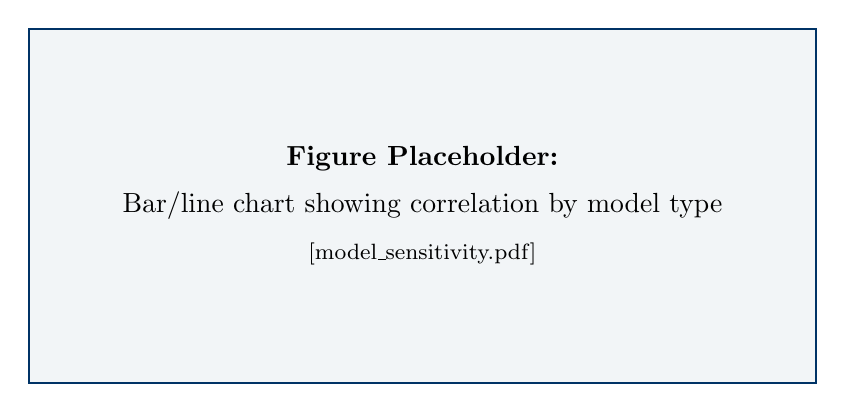
\begin{tikzpicture}
\draw[thick,kaistblue,fill=kaistblue!5] (0,0) rectangle (10,4.5);
\node[align=center] at (5,2.25) {
    \textbf{Figure Placeholder:}\\[0.5em]
    Bar/line chart showing correlation by model type\\[0.5em]
    \footnotesize{[model\_sensitivity.pdf]}
};
\end{tikzpicture}
\end{center}

\vspace{0.5em}

\begin{columns}
\begin{column}{0.5\textwidth}
\centering
\begin{tabular}{lc}
\toprule
\textbf{Model} & \textbf{Correlation} ($\rho$) \\
\midrule
\textbf{LightGBM} & \textbf{0.833} \\
CatBoost & 0.667 \\
XGBoost & 0.548 \\
Random Forest & 0.300 \\
\bottomrule
\end{tabular}
\end{column}

\begin{column}{0.5\textwidth}
\textbf{Interpretation:}
\begin{itemize}
    \item Gradient boosting methods show stronger correlation
    \item LightGBM: Best diagnostic signal
    \item Random Forest: Weaker (ensemble averaging)
\end{itemize}
\end{column}
\end{columns}

\end{frame}

%==============================================================================
% THEORETICAL FOUNDATION (Slides 17-18)
%==============================================================================

\begin{frame}{Theoretical Foundation}

\begin{theorem}[APS Score Bound Under Shift]
Let $\mathcal{H}$ be the SHAP concentration and $\delta_j$ the shift magnitude in feature $j$. Under mild regularity conditions, the expected APS score deviation satisfies:
$$\mathbb{E}[|s_{\text{test}} - s_{\text{cal}}|] \leq C \cdot g(\mathcal{H}) \cdot \|\boldsymbol{\delta}\|_2$$
where $g(\mathcal{H})$ is \alert{monotonically increasing} in $\mathcal{H}$.
\end{theorem}

\vspace{1em}

\textbf{Key implications:}
\begin{enumerate}
    \item Higher concentration $\Rightarrow$ larger score perturbation bounds
    \item Score perturbation $\Rightarrow$ coverage deviation (via quantile shift)
    \item \alert{Concentration acts as a ``fragility amplifier''}
\end{enumerate}

\vspace{0.5em}
\centering
\textit{Full proof in paper Appendix A}
\end{frame}

%------------------------------------------------------------------------------

\begin{frame}{Intuition Behind the Theorem}

\begin{center}
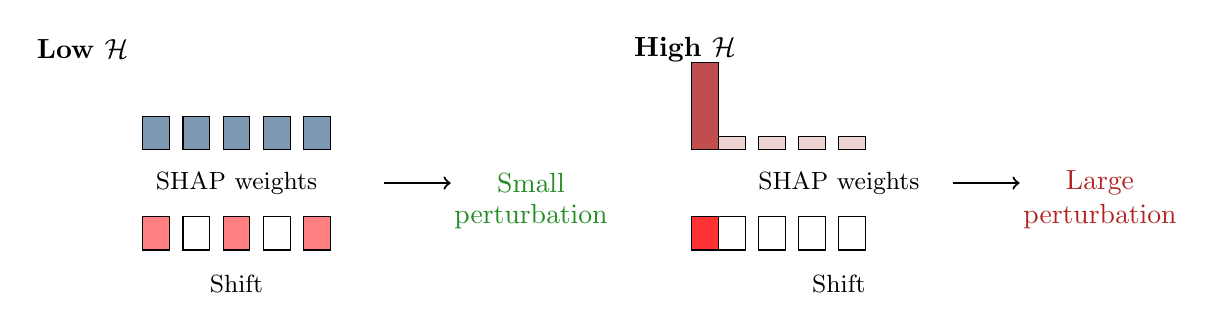
\begin{tikzpicture}[scale=0.85]
% Left: Low concentration
\node at (-0.5,4) {\textbf{Low $\mathcal{H}$}};

% Feature vector (uniform)
\foreach \i in {1,...,5} {
    \draw[fill=kaistblue!50] (\i*0.6-0.2,2.5) rectangle (\i*0.6+0.2,3);
}
\node at (1.8,2) {\small SHAP weights};

% Shift vector
\foreach \i/\c in {1/red,2/white,3/red,4/white,5/red} {
    \draw[fill=\c!50] (\i*0.6-0.2,1) rectangle (\i*0.6+0.2,1.5);
}
\node at (1.8,0.5) {\small Shift};

% Result
\draw[->,thick] (4,2) -- (5,2);
\node at (6.2,2) {\textcolor{successgreen}{Small}};
\node at (6.2,1.5) {\textcolor{successgreen}{perturbation}};

% Right: High concentration
\node at (8.5,4) {\textbf{High $\mathcal{H}$}};

% Feature vector (concentrated)
\draw[fill=alertred!80] (8.8-0.2,2.5) rectangle (8.8+0.2,3.8);
\foreach \i in {2,...,5} {
    \draw[fill=alertred!20] (8+\i*0.6-0.2,2.5) rectangle (8+\i*0.6+0.2,2.7);
}
\node at (10.8,2) {\small SHAP weights};

% Shift vector (hitting dominant feature)
\draw[fill=red!80] (8.8-0.2,1) rectangle (8.8+0.2,1.5);
\foreach \i in {2,...,5} {
    \draw[fill=white] (8+\i*0.6-0.2,1) rectangle (8+\i*0.6+0.2,1.5);
}
\node at (10.8,0.5) {\small Shift};

% Result
\draw[->,thick] (12.5,2) -- (13.5,2);
\node at (14.7,2) {\textcolor{alertred}{Large}};
\node at (14.7,1.5) {\textcolor{alertred}{perturbation}};
\end{tikzpicture}
\end{center}

\vspace{0.5em}

\begin{block}{The Amplification Mechanism}
When shift hits the dominant feature in a concentrated model, the weighted impact is much larger than when shift is spread across a model with uniform reliance.
\end{block}

\end{frame}

%==============================================================================
% PRACTICAL FRAMEWORK (Slides 19-20)
%==============================================================================

\begin{frame}{Operational Framework: 3-Step Protocol}

\begin{center}
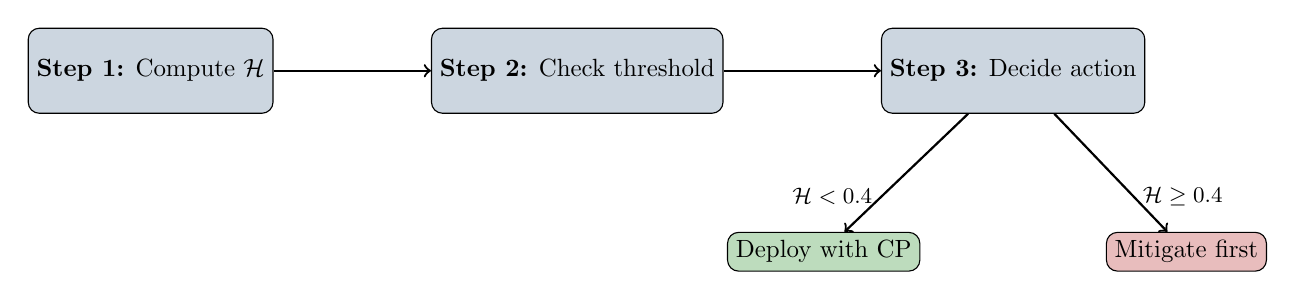
\begin{tikzpicture}[node distance=2cm, scale=0.9, every node/.style={scale=0.9}]
% Nodes
\node[draw, rounded corners, fill=kaistblue!20, minimum width=3cm, minimum height=1.2cm] (step1) {\textbf{Step 1:} Compute $\mathcal{H}$};
\node[draw, rounded corners, fill=kaistblue!20, minimum width=3cm, minimum height=1.2cm, right=of step1] (step2) {\textbf{Step 2:} Check threshold};
\node[draw, rounded corners, fill=kaistblue!20, minimum width=3cm, minimum height=1.2cm, right=of step2] (step3) {\textbf{Step 3:} Decide action};

% Arrows
\draw[->,thick] (step1) -- (step2);
\draw[->,thick] (step2) -- (step3);

% Decision outcomes
\node[draw, rounded corners, fill=successgreen!30, below left=1.5cm and -0.5cm of step3] (safe) {Deploy with CP};
\node[draw, rounded corners, fill=alertred!30, below right=1.5cm and -0.5cm of step3] (unsafe) {Mitigate first};

\draw[->,thick] (step3) -- node[left,pos=0.7] {\small $\mathcal{H} < 0.4$} (safe);
\draw[->,thick] (step3) -- node[right,pos=0.7] {\small $\mathcal{H} \geq 0.4$} (unsafe);
\end{tikzpicture}
\end{center}

\vspace{1em}

\begin{alertblock}{The 40\% Threshold}
Empirically, $\mathcal{H} \geq 0.40$ indicates elevated vulnerability to coverage failure under distribution shift.
\end{alertblock}

\end{frame}

%------------------------------------------------------------------------------

\begin{frame}{Mitigation Strategies}

\textbf{When SHAP Concentration exceeds threshold:}

\begin{columns}
\begin{column}{0.45\textwidth}
\textbf{1. Feature Engineering}
\begin{itemize}
    \item Diversify signal sources
    \item Reduce dominant feature reliance
\end{itemize}

\vspace{0.5em}

\textbf{2. Model Regularization}
\begin{itemize}
    \item Feature dropout
    \item Ensemble with diverse subsets
\end{itemize}

\vspace{0.5em}

\textbf{3. Monitoring}
\begin{itemize}
    \item Track $C$ over time
    \item Alert on threshold violations
\end{itemize}
\end{column}

\begin{column}{0.55\textwidth}
% Monitoring Framework Figure

\includegraphics[width=\textwidth]{figures/fig4_monitoring.jpg}
\end{column}
\end{columns}

\vspace{0.5em}
\centering
\fbox{\textbf{Key:} Address concentration \textit{before} deployment, not after failure}
\end{frame}

%==============================================================================
% LIMITATIONS & FUTURE WORK (Slides 21-22)
%==============================================================================

\begin{frame}{Limitations}

\begin{columns}
\begin{column}{0.5\textwidth}
\textbf{Current Limitations:}

\vspace{0.5em}

\begin{enumerate}
    \item \textbf{Tabular focus}
    \begin{itemize}
        \item Tested primarily on tabular data
        \item Extension to images/text needs study
    \end{itemize}

    \vspace{0.5em}

    \item \textbf{SHAP computation cost}
    \begin{itemize}
        \item TreeSHAP efficient for GBMs
        \item Deep learning: KernelSHAP slower
    \end{itemize}

    \vspace{0.5em}

    \item \textbf{Threshold calibration}
    \begin{itemize}
        \item 40\% is empirical
        \item May vary by domain
    \end{itemize}
\end{enumerate}
\end{column}

\begin{column}{0.5\textwidth}
\textbf{Scope Clarifications:}

\vspace{0.5em}

\begin{itemize}
    \item Diagnostic tool, not a fix
    \item Requires access to calibration data
    \item Correlation $\neq$ causation (but theory supports mechanism)
    \item Model-specific: works best with tree ensembles
\end{itemize}

\vspace{1em}

\textcolor{gray}{\footnotesize Note: We do not claim SHAP concentration \textit{causes} failures; it \textit{indicates} vulnerability.}
\end{column}
\end{columns}

\end{frame}

%------------------------------------------------------------------------------

\begin{frame}{Future Directions}

\begin{columns}
\begin{column}{0.33\textwidth}
\centering
\textbf{Extensions}\\[0.5em]
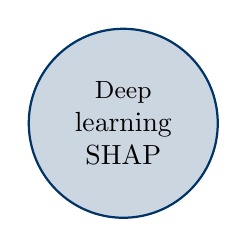
\begin{tikzpicture}
\draw[thick,kaistblue,fill=kaistblue!20] (0,0) circle (1.2);
\node[align=center] at (0,0) {\small Deep\\learning\\SHAP};
\end{tikzpicture}
\\[0.5em]
\footnotesize{Gradient-based explanations for neural networks}
\end{column}

\begin{column}{0.33\textwidth}
\centering
\textbf{Automation}\\[0.5em]
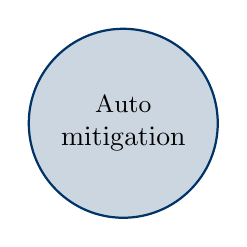
\begin{tikzpicture}
\draw[thick,kaistblue,fill=kaistblue!20] (0,0) circle (1.2);
\node[align=center] at (0,0) {\small Auto\\mitigation};
\end{tikzpicture}
\\[0.5em]
\footnotesize{Automatic feature engineering to reduce $\mathcal{H}$}
\end{column}

\begin{column}{0.33\textwidth}
\centering
\textbf{Theory}\\[0.5em]
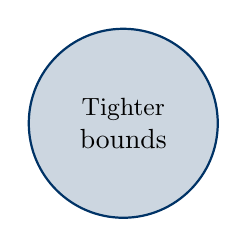
\begin{tikzpicture}
\draw[thick,kaistblue,fill=kaistblue!20] (0,0) circle (1.2);
\node[align=center] at (0,0) {\small Tighter\\bounds};
\end{tikzpicture}
\\[0.5em]
\footnotesize{Distribution-specific coverage bounds}
\end{column}
\end{columns}

\vspace{1.5em}

\textbf{Open Questions:}
\begin{itemize}
    \item Can we design models that are \textit{intrinsically} low-concentration?
    \item Relationship to other robustness notions (adversarial, OOD)?
    \item Online/streaming conformal prediction with concentration monitoring?
\end{itemize}

\end{frame}

%==============================================================================
% CONCLUSION (Slide 23)
%==============================================================================

\begin{frame}{Conclusion}

\begin{center}
\Large
\textbf{SHAP Concentration: A Pre-Deployment Diagnostic\\for Conformal Prediction Vulnerability}
\end{center}

\vspace{1em}

\begin{columns}
\begin{column}{0.6\textwidth}
\textbf{Key Contributions:}
\begin{enumerate}
    \item \alert{Predictive metric:} SHAP concentration correlates with coverage failure ($\rho = 0.853$)

    \item \alert{Theoretical grounding:} Monotonic bound on score perturbation

    \item \alert{Practical protocol:} 3-step framework with 40\% threshold
\end{enumerate}

\vspace{1em}

\textbf{Impact:}\\
Enables \textit{proactive} identification of vulnerable deployments \textbf{before} failures occur
\end{column}

\begin{column}{0.4\textwidth}
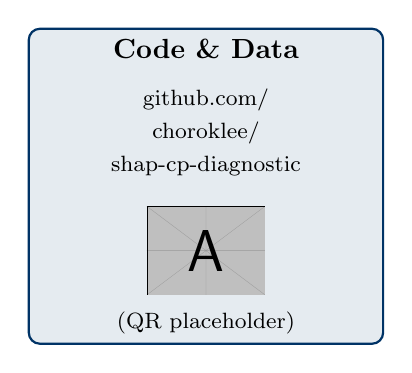
\begin{tikzpicture}
\draw[thick,kaistblue,fill=kaistblue!10,rounded corners] (0,0) rectangle (4.5,4);
\node[align=center] at (2.25,2) {
    \textbf{Code \& Data}\\[0.5em]
    \footnotesize{github.com/}\\
    \footnotesize{choroklee/}\\
    \footnotesize{shap-cp-diagnostic}\\[1em]
    \includegraphics[width=1.5cm]{example-image-a}\\
    \footnotesize{(QR placeholder)}
};
\end{tikzpicture}
\end{column}
\end{columns}

\vspace{0.5em}
\centering
\textbf{Thank you!} \quad Questions?
\end{frame}

%==============================================================================
% BACKUP SLIDES (Slides 24-26)
%==============================================================================

\begin{frame}[noframenumbering]{Backup: Full Results Table}

\begin{center}
\scriptsize
\begin{tabular}{llcccc}
\toprule
\textbf{Domain} & \textbf{Task} & \textbf{$C$ (\%)} & \textbf{Test Cov.} & \textbf{Drop (pp)} & \textbf{Shift} \\
\midrule
SALT & s-payterms & 54.2 & 13.7\% & 77.1 & Temporal \\
SALT & s-shipcond & 50.7 & 21.8\% & 71.6 & Temporal \\
SALT & i-shippoint & 48.8 & 72.7\% & 18.5 & Temporal \\
SALT & s-group & 47.3 & 12.4\% & 71.2 & Temporal \\
SALT & s-office & 42.6 & 99.9\% & 0.1 & Temporal \\
SALT & i-incoterms & 28.9 & 83.7\% & 11.3 & Temporal \\
SALT & i-plant & 23.9 & 81.4\% & 10.6 & Temporal \\
SALT & s-incoterms & 23.7 & 87.0\% & 8.5 & Temporal \\
\midrule
Covertype & Geographic & 49.8 & 8.2\% & \textcolor{alertred}{81.8} & Geographic \\
Gas Sensor & Temporal & 7.3 & Robust & --- & Temporal \\
KDDCup99 & Attack dist. & 21.1 & Variable & 15.9 & Distribution \\
PAMAP2 & Subject & 19.2 & Robust & --- & Population \\
\bottomrule
\end{tabular}
\end{center}

\vspace{0.3em}
\footnotesize{$C$ = SHAP Concentration (top-1/total). pp = percentage points drop from 90\% target.\\
Robust = coverage maintained near target. Variable = high seed variance.}

\end{frame}

%------------------------------------------------------------------------------

\begin{frame}[noframenumbering]{Backup: SHAP Computation Details}

\textbf{TreeSHAP Implementation:}

\begin{itemize}
    \item Used SHAP library v0.42.1
    \item TreeExplainer for gradient boosting models
    \item Exact SHAP values (not approximate)
    \item Computation time: $\sim$1 second per 1,000 samples
\end{itemize}

\vspace{1em}

\textbf{Aggregation Method:}
$$|\phi_j| = \frac{1}{n \cdot K} \sum_{i=1}^{n} \sum_{k=1}^{K} |\phi_j^{(k)}(x_i)|$$

\begin{itemize}
    \item Average absolute SHAP across samples and classes
    \item Normalization ensures $\sum_j p_j = 1$
    \item Entropy computed with natural log
\end{itemize}

\vspace{1em}

\textbf{Robustness:}
\begin{itemize}
    \item Results stable across calibration set sizes (1K--10K)
    \item Bootstrap confidence intervals included in paper
\end{itemize}

\end{frame}

%------------------------------------------------------------------------------

\begin{frame}[noframenumbering]{Backup: Statistical Analysis}

\textbf{Correlation Analysis:}

\vspace{0.5em}

\begin{columns}
\begin{column}{0.5\textwidth}
\textbf{Spearman Correlation:}
\begin{itemize}
    \item Overall: $\rho = 0.853$ ($p < 0.001$)
    \item SALT only: $\rho = 0.833$ ($p = 0.010$)
    \item 95\% CI: [0.71, 0.94]
\end{itemize}

\vspace{1em}

\textbf{Why Spearman?}
\begin{itemize}
    \item Robust to outliers
    \item Captures monotonic relationships
    \item Appropriate for ordinal patterns
\end{itemize}
\end{column}

\begin{column}{0.5\textwidth}
\textbf{Comparison with Baselines:}

\vspace{0.5em}
\begin{tabular}{lcc}
\toprule
\textbf{Metric} & $\rho$ & $p$-value \\
\midrule
SHAP Conc. & 0.853 & $<$0.001 \\
MMD & 0.19 & 0.48 \\
C2ST & 0.15 & 0.58 \\
PSI & 0.12 & 0.66 \\
KL Div. & 0.21 & 0.43 \\
\bottomrule
\end{tabular}

\vspace{0.5em}
\footnotesize{Only SHAP concentration achieves statistical significance}
\end{column}
\end{columns}

\end{frame}

\end{document}
